Los marinos miden la dirección de una línea por medio del ángulo que forma con una dirección de referencia. Algunos de estos ángulos tienen un nombre específico (figura \ref{fg:rumbo-demora}):  
\begin{itemize}
\item \emph{Rumbo} ($R$) es el ángulo que forma la dirección que sigue el barco con la línea Norte-Sur. Se mide de 0º a 360º en el sentido de las agujas del reloj. 
\item  \emph{Demora} ($D$) o \emph{acimut} ($Z$) es el ángulo que forma la visual a un objeto con la línea Norte-Sur. Se suele usar la palabra \emph{demora} cuando se trata de un objeto terrestre, y \emph{acimut} cuando se refiere a un astro. Se mide también de 0º a 360º en el sentido de las agujas del reloj. 
\item \emph{Marcación} ($M$) es el ángulo que forma la visual a un objeto con la dirección que sigue el barco. Se mide de 0º a 180º hacia estribor (\emph{Er}) o babor (\emph{Br}).
La marcación se relaciona con el rumbo y la demora mediante la fórmula: 
\begin{equation}
D = R + M
\end{equation}
Las marcaciones a estribor se consideran positivas, y hacia babor negativas.
\end{itemize}

\begin{figure}[htbp]
\begin{center}
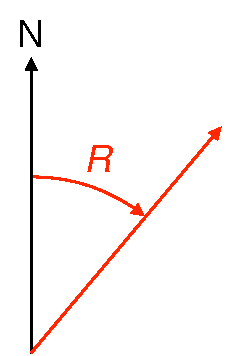
\includegraphics[scale=0.45]{rumbo}\\
\caption{Rumbo, demora y marcación}
\label{fg:rumbo-demora}
\end{center}
\end{figure}

Esta forma de medir los rumbos, denominada \emph{circular}, es la que se emplea de forma generalizada en la actualidad (figura \ref{fg:circular-cuadrantal}). Los rumbos y demoras se escriben siempre con tres cifras, aunque su valor sea menor de 100º (por ejemplo, 005º o 045º).  

A veces todavía se dan los rumbos en el sistema \emph{cuadrantal}, cada vez más en desuso. En este sistema los rumbos se miden de 0º a 90º desde el Norte o el Sur hacia el Este o el Oeste. Los rumbos cuadrantales se escriben con dos cifras, precedidos del punto (N o S) a partir del cual se toman, y seguidos del punto (E u W) hacia el que se orientan. Para pasar de rumbos cuadrantales a circulares, o viceversa, basta tener en cuenta la figura  \ref{fg:circular-cuadrantal}.

\begin{ejemplo}
El rumbo cuadrantal S 70º E equivale al 110º circular (figura \ref{fg:ejemplo-cuadrantal}). El rumbo WSW equi- 
vale al 247,5º circular. 
\end{ejemplo}

Una forma tradicional de medir los ángulos es la denominada  \emph{por cuartas}, que resulta de la antigua división de la rosa de los vientos (figura \ref{fg:circular-cuadrantal}). En este sistema se divide el horizonte en primer lugar en cuatro partes, tomando las direcciones correspondientes a los puntos cardinales Norte, Sur, Este y Oeste. Cada una de estas partes se divide a su vez en dos, dando lugar a los \emph{rumbos laterales}: Nordeste (NE), Sureste (SE), Suroeste (SW) y Noroeste (NW). Una nueva subdivisión da lugar a los \emph{rumbos colaterales}: Nornordeste (NNE), Estenordeste (ENE), etc. Por último, se divide el horizonte en 32  \emph{cuartas}, dando lugar a los rumbos Norte cuarta al Este (N 1/4 E), etc. Una cuarta vale, por tanto, 22,5º (1/32 de 360º).

El cuadro \ref{tb:rumbos} contiene los nombres de los 32 rumbos y su equivalencia en el sistema circular y cuadrantal. 


\begin{figure}[tbp]
\begin{center}
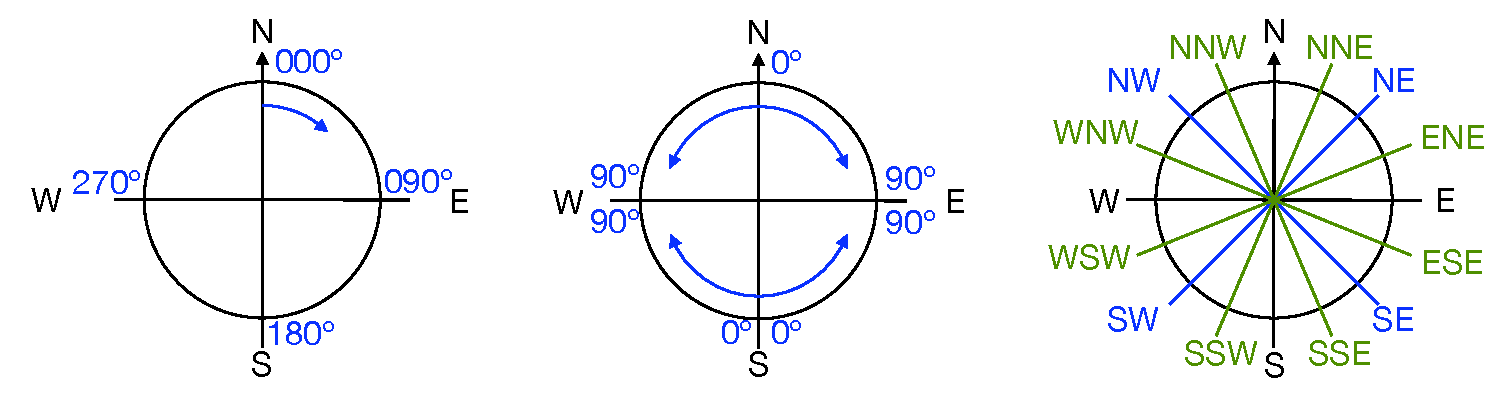
\includegraphics[scale=0.45]{rumbos}\\
\caption{Rumbo circular, cuadrantal y por cuartas}
\label{fg:circular-cuadrantal}
\end{center}
\end{figure}

\begin{table}[htbp]
\caption{Rumbos de la rosa de los vientos}
\begin{center}
\begin{tabular}{llll}
\multicolumn{2}{c}{\textbf{Rumbo}} & \textbf{Circular} & \textbf{Cuadrantal} \\
\hline
N & Norte & 000º & N \\
N 1/4 E & Norte cuarta Este & 022,5º & N 22,5º E \\
NNE      & Nornordeste & 045º & N 45º E \\
NE 1/4 N & Nordeste cuarta Norte & 067,5º & N 67,5º E \\

\hline
\end{tabular}
\end{center}
\label{tb:rumbos}
\end{table}%


Las líneas que forman un ángulo constante con los meridianos (es decir con el Norte) se llaman \emph{líneas loxodrómicas}. Los barcos suelen seguir líneas loxodrómicas en su navegación, ya que para ello basta con mantener un rumbo constante. 

-------------------------------------------------------------------------------------
%-------------------------------------------------------------------------------
\subsubsection{Latitudes aumentadas }

 \index{carta!mercatoriana!latitudes aumentadas}

Aunque la escala de una carta mercatoriana varía con la latitud, podemos considerarla 
constante si nos fijamos sólo en una zona suficientemente pequeña de la carta. En este 
caso la escala debe ser la misma a lo largo de los meridianos y de los paralelos, con el fin 
de mantener el valor de los ángulos medidos sobre la superficie terrestre, y por tanto el 
carácter conforme de la proyección. 

\begin{figure}[btp]
\begin{center}
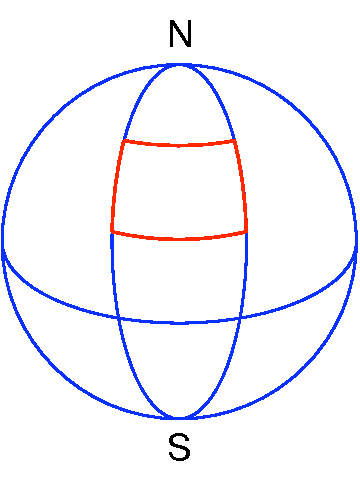
\includegraphics[scale=0.45]{convergencia}\\
\caption{Convergencia de los meridianos.}
\label{fg:convergencia}
\end{center}
\end{figure}

La longitud de un arco de 1’ de meridiano es prácticamente igual en todas las latitudes, 
salvo una pequeña diferencia debida a la falta de esfericidad de la Tierra. Esta distancia es 
aproximadamente igual a 1 milla náutica, es decir 1852\,m. Por el contrario, un arco de
 1’~de paralelo sólo mide 1 milla en el Ecuador. A medida que se avanza hacia latitudes más 
altas, los meridianos se van acercando (figura~\ref{fg:convergencia}), por lo que la longitud de los paralelos 
va disminuyendo con la latitud, de tal manera que en la latitud $\phi$ la longitud de un arco de 
1’ de paralelo es igual a $\cos\, \phi$ millas. Por otra parte, en la proyección de Mercator la separación entre los meridianos es constante e independiente de la latitud. Por tanto, es necesario aumentar la escala en el sentido de la latitud para mantener la proporción entre la medida de los arcos de meridiano y de paralelo en todas las latitudes. Si consideramos un rectángulo de $\Delta \phi$ de latitud por $\Delta \lambda$ de longitud cuya esquina inferior izquierda tiene unas coordenadas $\phi, \lambda$, la relación entre los lados del rectángulo $(x, y)$ es: 

\begin{equation}
\frac{y}{x} = \frac{1}{\cos \phi} = \sec \phi
\label{eq:escala}
\end{equation}

Por tanto, en la proyección de Mercator la latitud se representa de forma que aparece «aumentada» con respecto a la longitud. La relación entre ambas es proporciona a la secante de la latitud.%
\footnote{La función secante es la inversa del coseno.} 

\begin{ejemplo}
 La figura \ref{fg:escalas-lat-long} muestra la representación en una carta mercatoriana de un rectángulo de 
1’ de latitud por 1’ de longitud situado en la latitud 38º 00’ N. Suponemos una escala de 1/50~000, por lo que 1' de latitud se representa mediante un segmento de $1852/50000 = 0.0037\,\mbox{m} = 37\, \mbox{mm}$,  que en la figura corresponde al lado vertical del rectángulo. La medida del lado horizontal es igual a $37 \cdot \cos 38º = 29.2\, \mbox{mm}$.
\end{ejemplo}

\begin{figure}[hbtp]
\begin{center}
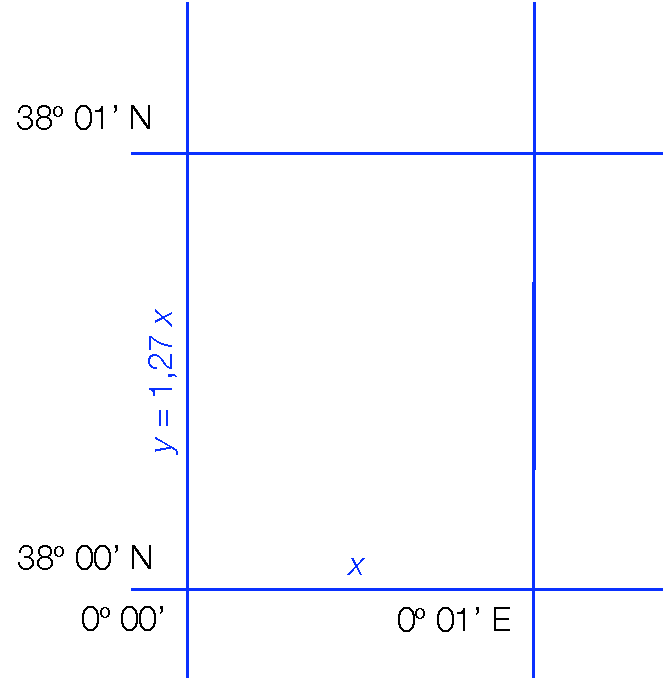
\includegraphics[scale=0.50]{escalas-lat-long}\\
\caption{Escalas de latitud y longitud.}
\label{fg:escalas-lat-long}
\end{center}
\end{figure}

%%%%%%%%%%%%%%%%%%%%%%%%%%%%%%%%%%%%%%%%%%%%

Hay que tener en cuenta, no obstante, que esta relación (ecuación \ref{eq:escala}) sólo es válida para zonas reducidas de la carta, en las que podemos suponer que la escala es constante. Por lo general se considera que esto es así si la diferencia de latitudes de la zona representada en la carta es menor que 1º. 
Cuando se consideran intervalos de latitud más amplios hay que recurrir al concepto de \emph{ latitud aumentada}. 
La latitud aumentada de un punto es la distancia que separa su representación en una carta mercatoriana del Ecuador. La latitud aumentada de un punto de latitud $\phi$ es igual a:
 
 \index{latitud!aumentada|textbf}

\begin{equation}
\phi_{a} = 7915.7 \ln \tan \left( 45º+ \frac{\phi}{2}\right)
\end{equation}

Esta función se obtiene suponiendo que la Tierra es esférica, por lo que puede ser 
necesario corregirla para el elipsoide de referencia de las cartas que se utilicen. 

